\section{Design}

The CLAS12 DAQ was designed as a pipeline-style, network-based system. The data taking process starts from the front-end components. Those components can have different hardware and software implementations, but have to follow certain requirements to be compatible with the rest of the system. Currently, the front-end components used are commercial VME/VXS crates, commercial Linux servers, and Jefferson Laboratory(JLAB)-designed VXS Trigger Processor boards (VTP). VTPs are installed in all of the VXS crates, but they are read out by the DAQ as independent components. All components receive a common 250~MHz clock distributed over OM3-rated parallel optic fibers. The same fiber system is used to distribute both the synchronization reset and trigger signals and to collect the busy signals from all front-end electronics.

All front-end components are connected via TCP sockets over ethernet to the Event Builder (EB) component. The EB is a multi-threaded program (C application) running on a multi-core Linux server. Most front end connections are 1 Gb links. However, for several components, that generate significant data rate, a 10 Gb ethernet connection is used.

Built events are output to the Event Transfer (ET) System. This multi-threaded program (C application) provides access to shared memory storage in a ring architecture where multiple data processing programs can be attached to process, filter or monitor data quality online. The ET system is typically run on the same server as the EB, but it can also be used to distribute events to a sequential chain of ET servers to increase the aggregate data processing power.

The last component in the data chain is the Event Recorder (ER). This multi-threaded program receives data from the ET system and records it to the disk. A multi-stream mode is available, that allows several files to be written in parallel to the same or different disk partitions to increase writing performance. The event order in multi-stream mode is preserved. The CLAS12 DAQ system diagram is shown in Fig.~\ref{fig:DAQdiagram}.

\begin{figure}[hbt]
	\centering
	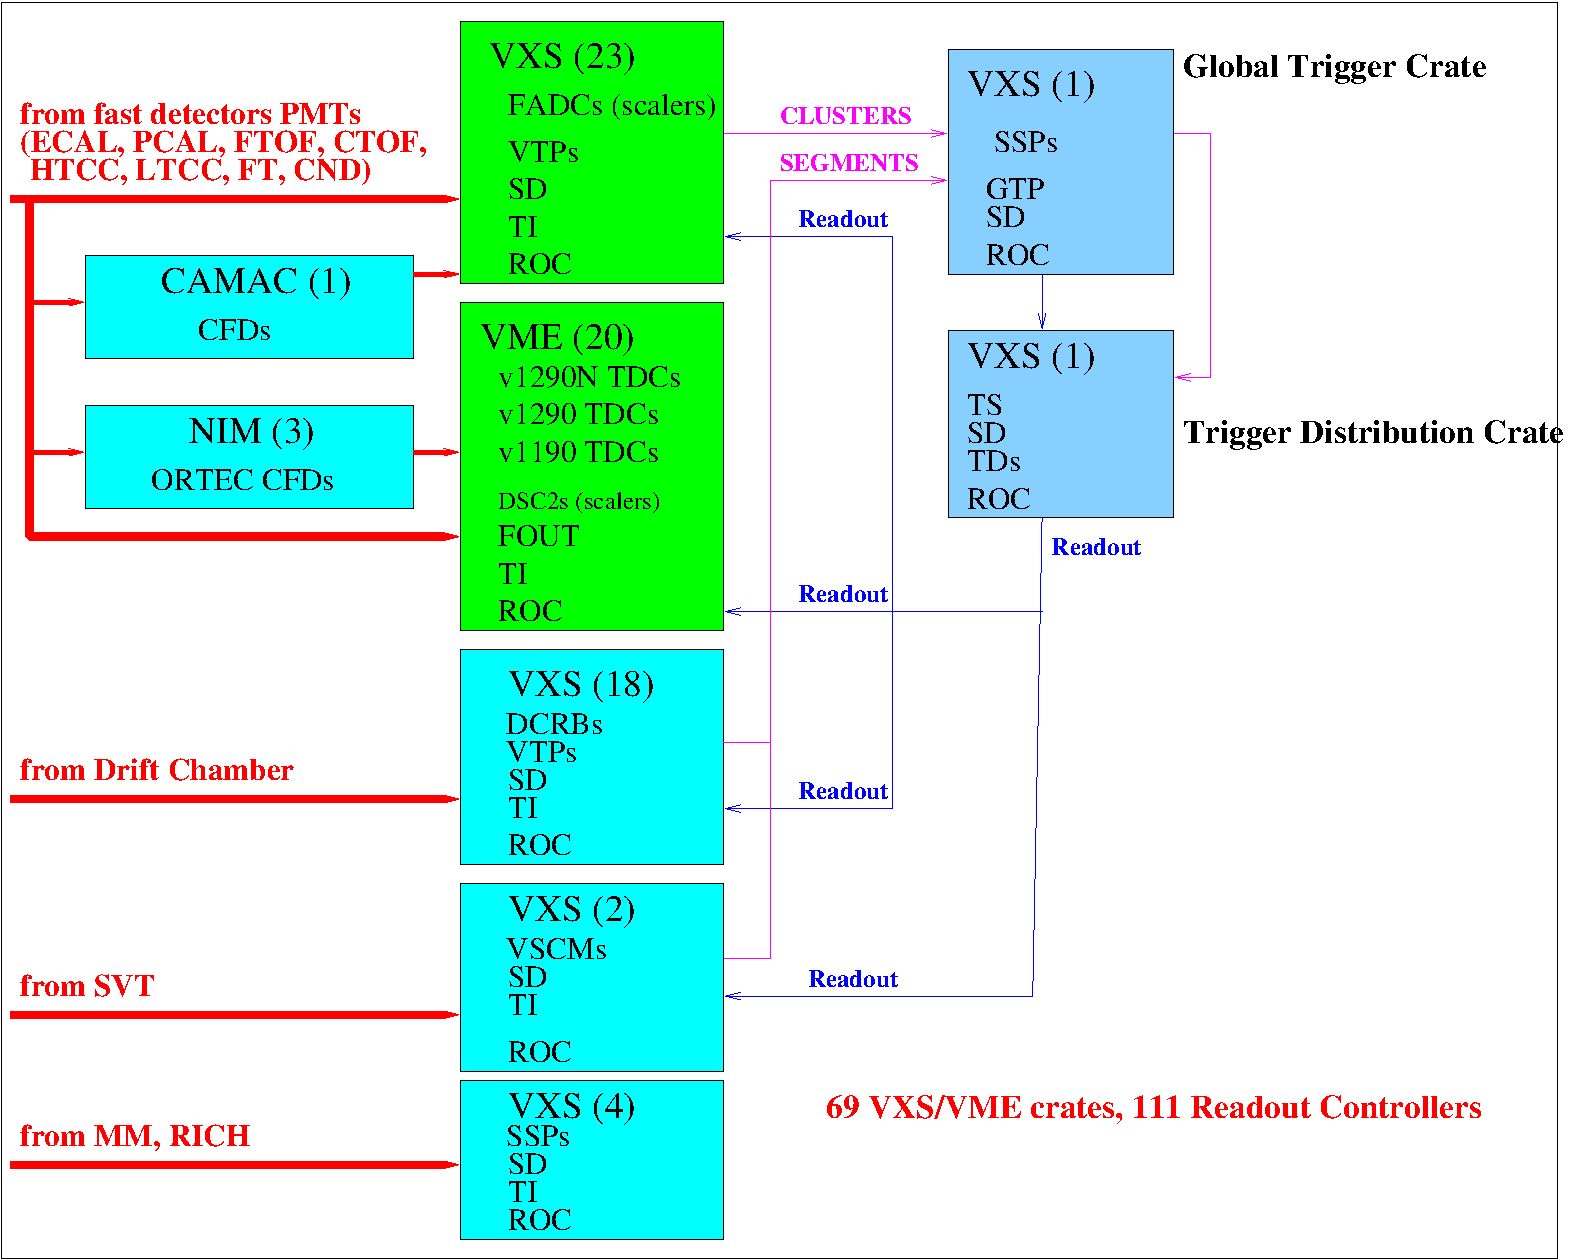
\includegraphics[width=1.0\columnwidth,keepaspectratio]{img/CLAS12_HARDWARE_2.pdf}
	\caption{Diagram of the CLAS12 Data Aquisition System. }
	\label{fig:DAQdiagram}
\end{figure}

